\section{Renderer Accuracy Validation}

There are many different render engines available to generate imagery of a simulated scene.  Before using a render engine to analyze surface reconstructions a series of validation experiments should be performed to ensure that the render engine is generating imagery as expected.  These validation experiments are performed to ensure that any resultant error in an uncertainty analysis is due to SFM algorithm, not inaccurate rendering.  In this paper, we present an assessment and validation using Blender Internal Render Engine, but this validation methodology could be applied to any render engine.  Note that there is no experiment presented to validate that accuracy of the lighting as the radiometric accuracy of the lighting is not the focus of this experiment.  The authors recognize the render engine could also be validated by rigorously analyzing or developing the rendering source code, but believe these experiments provide a less time consuming methodology.

\subsection{Photogrammetric Projection Accuracy}
The first validation experiment is designed to ensure that the camera interior and exterior orientation are set accurately using a pinhole camera model.  This experiment is performed by creating a simple scene consisting of a 1000m$^3$ cube with a 10x10 black and white checkerboard pattern on each wall, as depicted in \figref{fig:checker}.   The black and white corner of each checkerboard corner is at a known 3D world coordinates.  A series of images are rendered using various camera rotations, translations, focal lengths, sensor sizes, and principal point coordinates.  To ensure that the images are rendered correctly, the coordinates of the checkerboard corners are calculated from the rendered imagery using a corner feature detector and compared to the expected coordinates of the targets using photogrammetric equations.  The difference between the image derived coordinates and the photogrammetric equation derived coordinates should have a mean of 0 in both dimensions, and a subpixel variance on the order of the accuracy of the image corner feature detector.  There should also be no correlation between the accuracy of the coordinate and the location of the coordinate in the image.\todo{is correlation necessary???}

\begin{figure}[H]
	\centering
	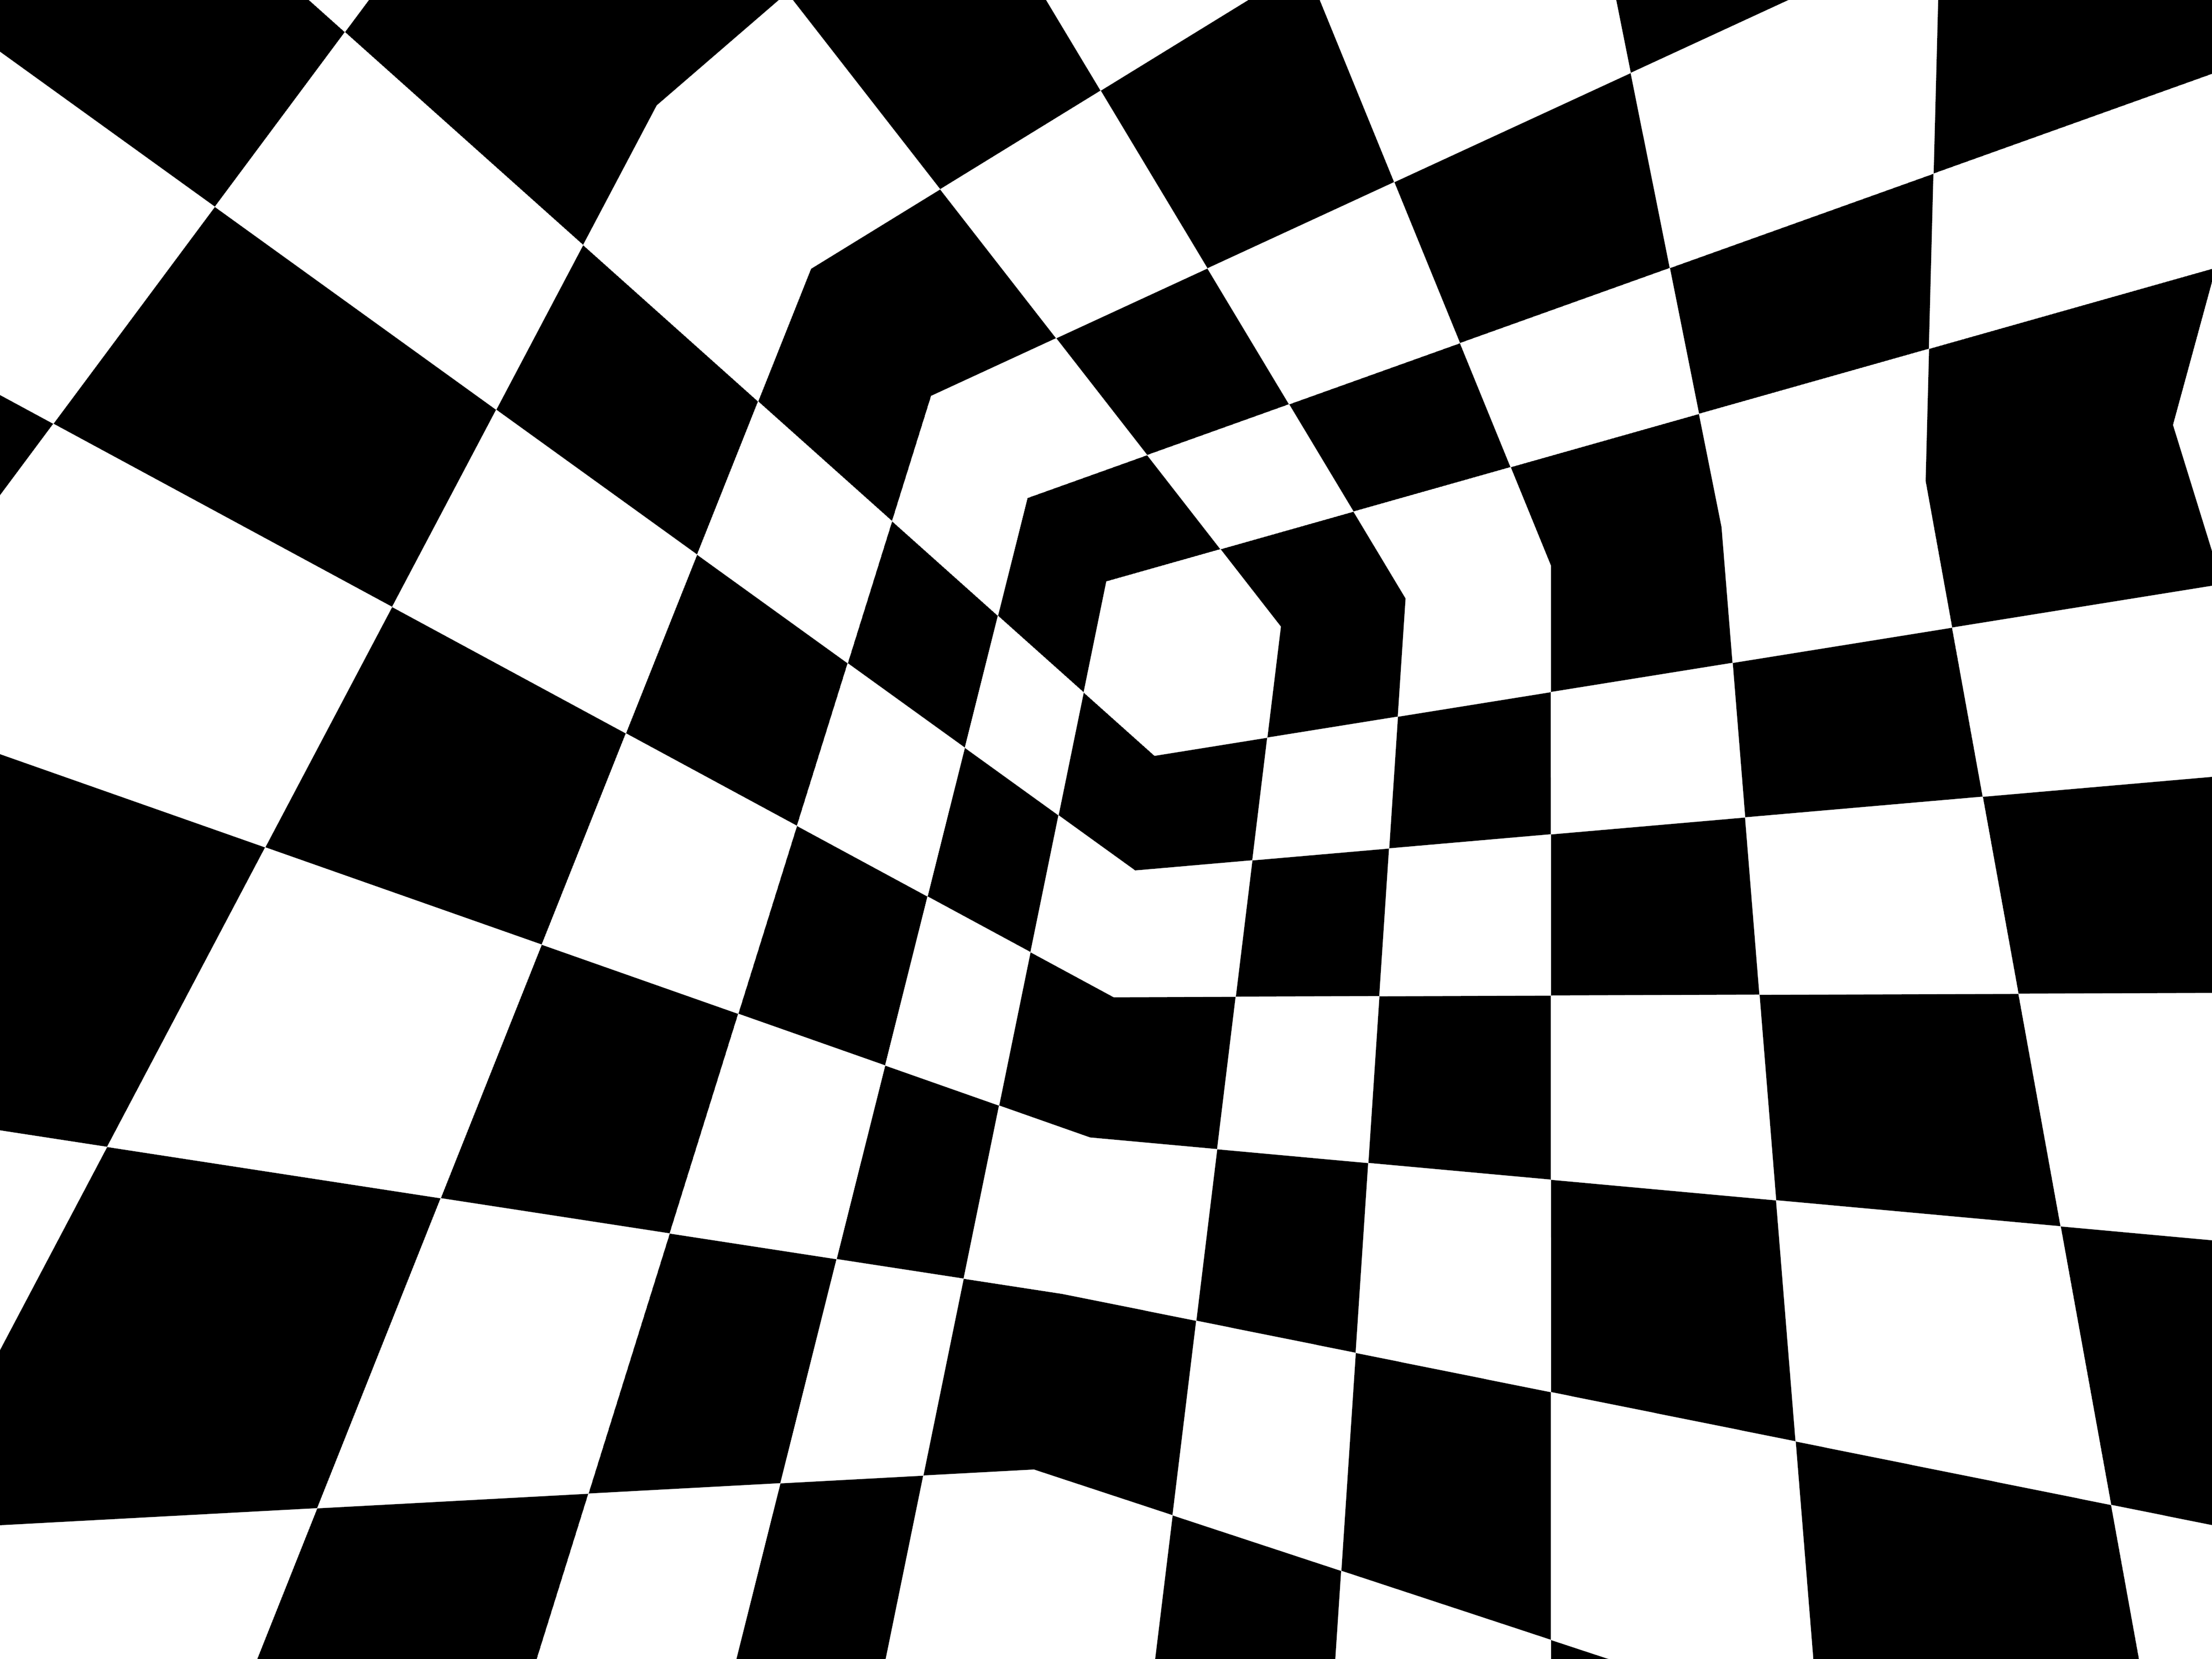
\includegraphics[height = 2in]{../fig/checkerRoom}
	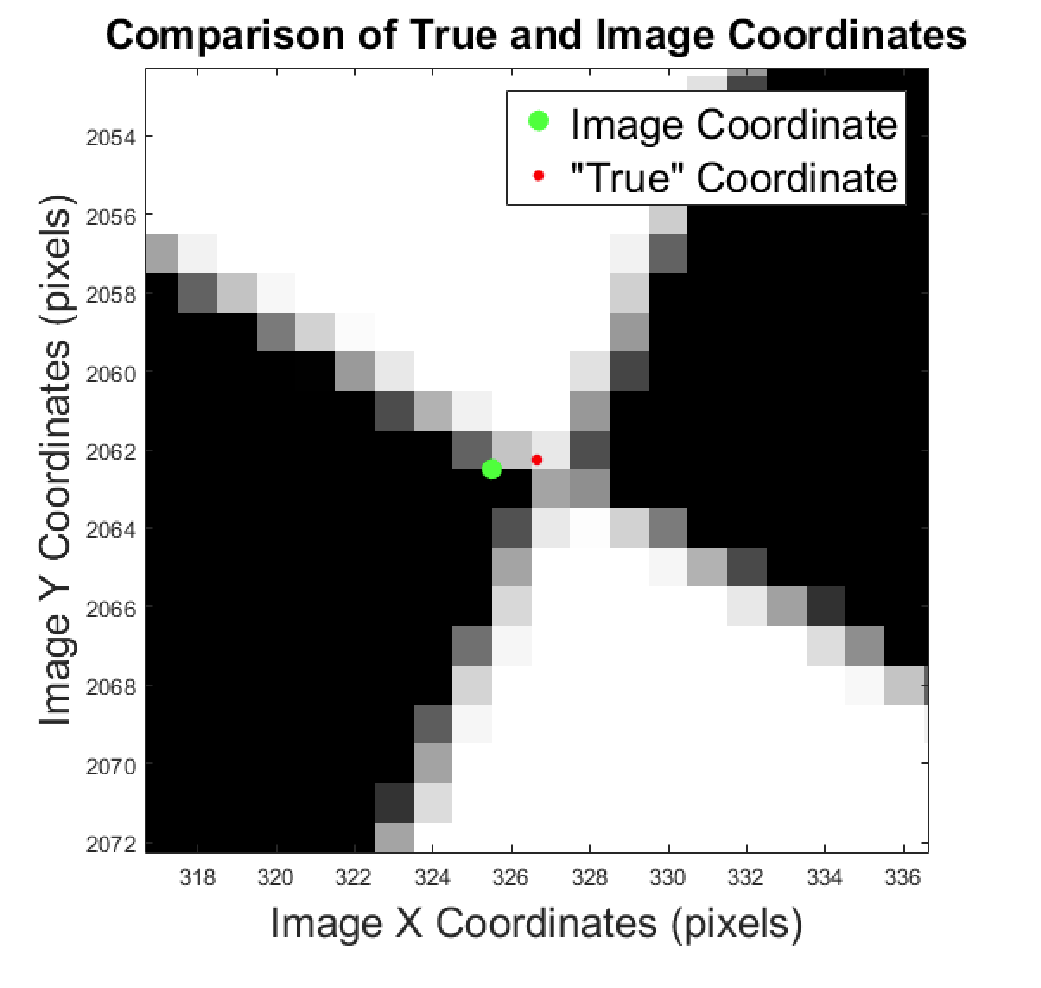
\includegraphics[height = 2in]{../fig/dPixZoom}
	\caption{A cube with a 10x10 checkerboard pattern on each wall is used to validate the photogrammetric accuracy of the Blender Internal Render Engine.}
	\label{fig:checker}
\end{figure}

To validate the photogrammetric projection accuracy of the Blender Internal Render Engine using this experiment, a 1000m$^3$ cube was placed with the centroid at the origin.  Five hundred images were rendered using five different interior orientations and random exterior orientations throughout the inside of the cube.  These parameters were input using the Blender Python API, and the distribution of each input parameter are shown in \tabref{tab:paramdist}.  The accuracy of the imagery was observed qualitatively by plotting the photogrammetric equation calculated points on the imagery in Matlab to ensure a rough accuracy.  Once the rough accuracy is confirmed, a nearest neighbor is used to develop correspondences between the Harris corner coordinates and the photogrammetric equation derived coordinates.  The mean and variance of the differences between the correspondences in each experiment are shown in \tabref{tab:deltas}.  \todo{again, correlation needed??}The correlation between the difference in x, y, and radius versus several parameters shows no statistically significant correlation.  The correlation results are summarized in \tabref{tab:correlations}.

% Table generated by Excel2LaTeX from sheet 'Parameter Distributions'
\begin{table}[htbp]
  \centering
  \caption{The position of the cameras used to render the imagery were uniformly distributed using parameters to full encompass every position and look angle within the box.  Note that the translation was kept 1 meter away from the edge of the box on all sides.}
    \begin{tabular}{lrrr}
    	\toprule
    Parameter & Minimum & Maximum & units \\
    \midrule
    Translation X, Y, Z & -4    & 4     & m \\
    Rotation Theta, Phi & 0     & 360   & degrees \\
    Rotation Omega & 0     & 180   & degrees \\
    \bottomrule
    \end{tabular}%
  \label{tab:paramdist}%
\end{table}%
% Table generated by Excel2LaTeX from sheet 'PixDeltas'
\begin{table}[htbp]
  \centering
  \caption{The difference between the Harris Corner detected corners and the expected position of the corners from the photogrammetry equations is assessed to ensure that the rendering algorithm are working correctly.  Note that the mean and variance of the difference between expected and detected are sub-pixel for each simulated camera, which suggests that the Blender Internal Renderer is accurate.}
    \begin{tabular}{lrrrrrrr}
      \toprule
      hFOV (\degree) & Horizontal & Vertical & \# Corners & mean $\Delta x$ & mean $\Delta y$ & var $\Delta x$ & var $\Delta y$ \\
    \midrule
    11.5  & 5184  & 3456  & 462   & -0.0163 & 0.0035 & 0.0855 & 0.0827 \\
    29.0  & 3264  & 2448  & 3538  & 0.0050 & 0.0078 & 0.0915 & 0.0776 \\
    36.3  & 5456  & 3632  & 4093  & 0.0016 & 0.0116 & 0.0652 & 0.0715 \\
    36.9  & 4608  & 3456  & 4491  & -0.0036 & 0.0041 & 0.0865 & 0.0705 \\
    46.8  & 4000  & 3000  & 7493  & 0.0033 & 0.0081 & 0.0797 & 0.0867 \\
    \bottomrule
    \end{tabular}%
  \label{tab:deltas}%
\end{table}%
% Table generated by Excel2LaTeX from sheet 'Correlations'
\begin{table}[htbp]
  \centering
  \caption{The correlation between the errors and the location in the frame of the image is also calculated to ensure there is no systematic offset introduced due to the rendering.  The Blender Internal Renderer shows no systematic biasing of the rendered image.}
    \begin{tabular}{llrrr}
    \toprule
    IV    & DV    & Slope & Bias  & Different than 0 slope 0 bias? \\
    \midrule
    x     & dx    &       &       & no \\
    y     & dx    &       &       & no \\
    r     & dx    &       &       & no \\
    x     & dy    &       &       & no \\
    y     & dy    &       &       & no \\
    r     & dy    &       &       & no \\
    \bottomrule
    \end{tabular}%
  \label{tab:correlations}%
\end{table}%

To ensure that the variance is not an artifact of the rendering, an experiment was performed to determine the expected accuracy of the Harris Corner detector.  1000 Simulated checkerboard patterns were generated with random rotations, translations, and skew to create a synthetic image dataset.  The known coordinates of the corners were compared to the coordinates calculated with the Harris Corner feature detector, and the results are shown in in \tabref{tab:harrisdeltas}.  \todo{reword??}From these results, the hypothesis that the variance of the rendered image coordinate error is statistically different than the variance of the simulated image coordinate error is rejected.  Therefore, all the variance can be statistically attributed to the Harris Feature Corner detection algorithm, rather than the render engine. 

% Table generated by Excel2LaTeX from sheet 'HarrisDeltas'
\begin{table}[htbp]
  \centering
  \caption{A checkerboard pattern is generated and then warped in Matlab before extracting the Harris Corner Features.  The difference between the known checkerboard corners and the Harris corner features are on the same order of magnitude as the differences in the rendered imagery simulation.  This suggests that the variance and mean offsets in the simulation are due to the uncertainty in the Harris Corner extraction, and not the renderer.}
    \begin{tabular}{lrrrrr}
   	\toprule
    Name  & \# Correspondences & dX & dY & var X & var Y \\
    \midrule
    Warped Imagery & 390204 & -0.0012 & 0.0075 & 0.0462 & 0.0474 \\
    \bottomrule
    \end{tabular}%
  \label{tab:harrisdeltas}%
\end{table}%


\subsection{Point Spread Function}
The second validation experiment ensures that there is no blurring applied to the rendered image.  Specifically, this test determines that the point spread function of the rendered imagery is a unit impulse.  This test is performed by simulating a white circular plane placed at a distance and size such that it exists in only one pixel.  The rendered image should therefore only contain white in the one pixel and not be blurred into any other pixels.  This test is particularly important when antialiasing is performed, as the supersampling pattern and filter used to combine the samples can sometimes create a blurring effect.  For example, the default antialiasing in blender uses a "distributed jitter" pattern and the Mitchel-Netrevali filter, which uses supersampled values from neighboring pixels to calculate a pixel value.  This effect can be seen in \figref{fig:aliasing}, where the intensity of the white plane is experienced in eight of the neighboring pixels, even though the sphere should only be visible in one pixel.  While this photogrammetric inaccuracy is minimal, the error could propagate into the resultant SFM derived pointcloud especially when fine scale textures with high gradient are used.

\begin{figure}[H]
	\centering
	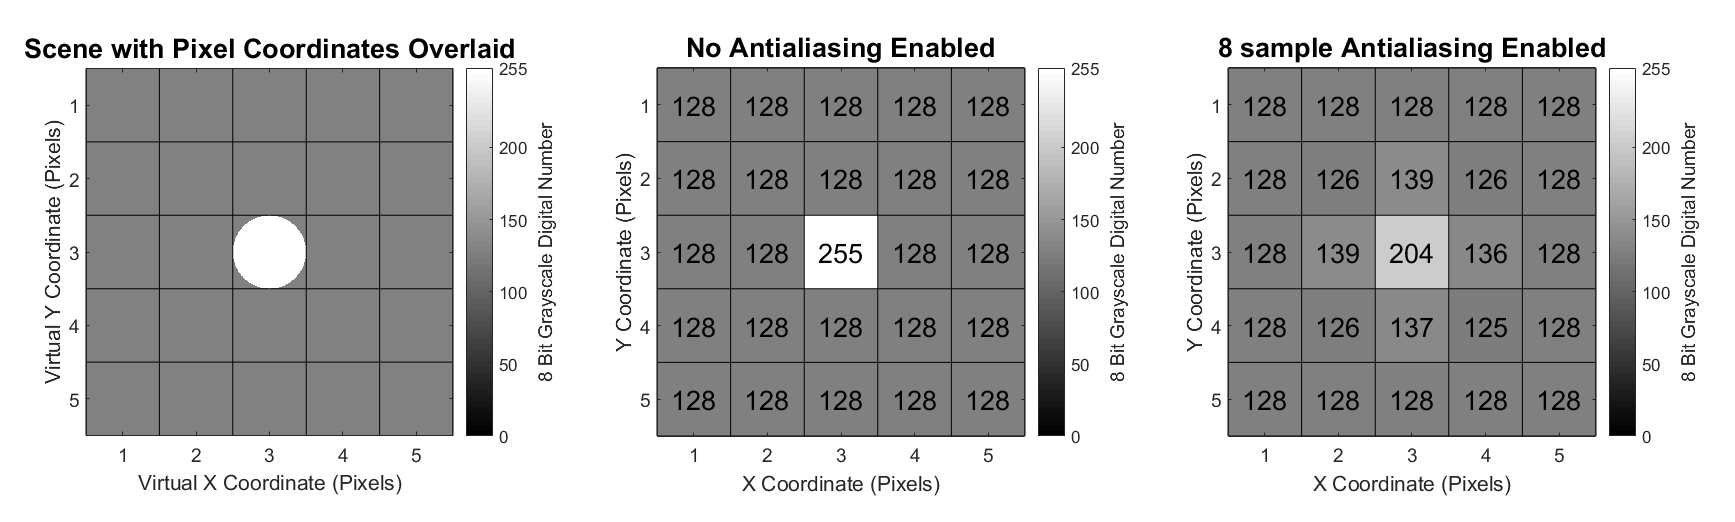
\includegraphics[height = 2in]{../fig/Antialiasing.png}
	\caption{A circular plane placed so it is encompassed by the viewing volume of only the central pixel (right) is rendered with the no antialiasing (middle) and with 8 sample antialiasing (right).  }
	\label{fig:aliasing}
\end{figure}

To validate the point spread function of the Blender Internal Render Engine, a sensor and scene are set up such that the geometry of the circular plane is only captured with one pixel in the render of a 5x5 pixel image.  This experiment ensures that any other pixels that contain white are an artifact of the rendering.  Rendered imagery is shown with and without antialiasing.  The antialiasing used is the default settings for the Blender Internal Render Engine (8 Samples, Mitchell-Netrevali filter).  The rendered image with no antialiasing contains no blurring of the image, while the antialiased image contains a slight amount of blurring.  The antialiased imagery renders a smoother, more photorealisitic imagery, and is deemed to be suitable for experimentation. \todo{Need to word this better... I contradict myself by saying antialiasing is bad}

\subsection{Texture Resolution}
The final validation experiment ensures that any textures applied to the objects in the scene are applied in a manner which maintains the resolution of the imagery.  This validation experiment is performed by rendering a texture on a flat plane and rendering an image that contains a small number of the texture pixels.  By qualitatively looking at the image, it should be clear that the desired number of pixels are in the frame, and no smoothing is being applied.  When rendering textures in computer graphics there is an option to perform interpolation of the texture, which yields a smoother texture.  An example of a texture with and without interpolation is shown in Figure X. 

To validate the texture resolution of the Blender Internal Render Engine a black and white checkerboard pattern where each checkerboard square is 1x1 texel is applied to a flat plane such that each texel represents a 10cm x 10cm square.  An image is rendered using a focal length and sensor size such that each texel is captured by 100 x 100 pixels.  The rendered image is qualitatively observed to ensure that the checkerboard is rendered for each pixel.   

\begin{figure}[H]
	\centering
	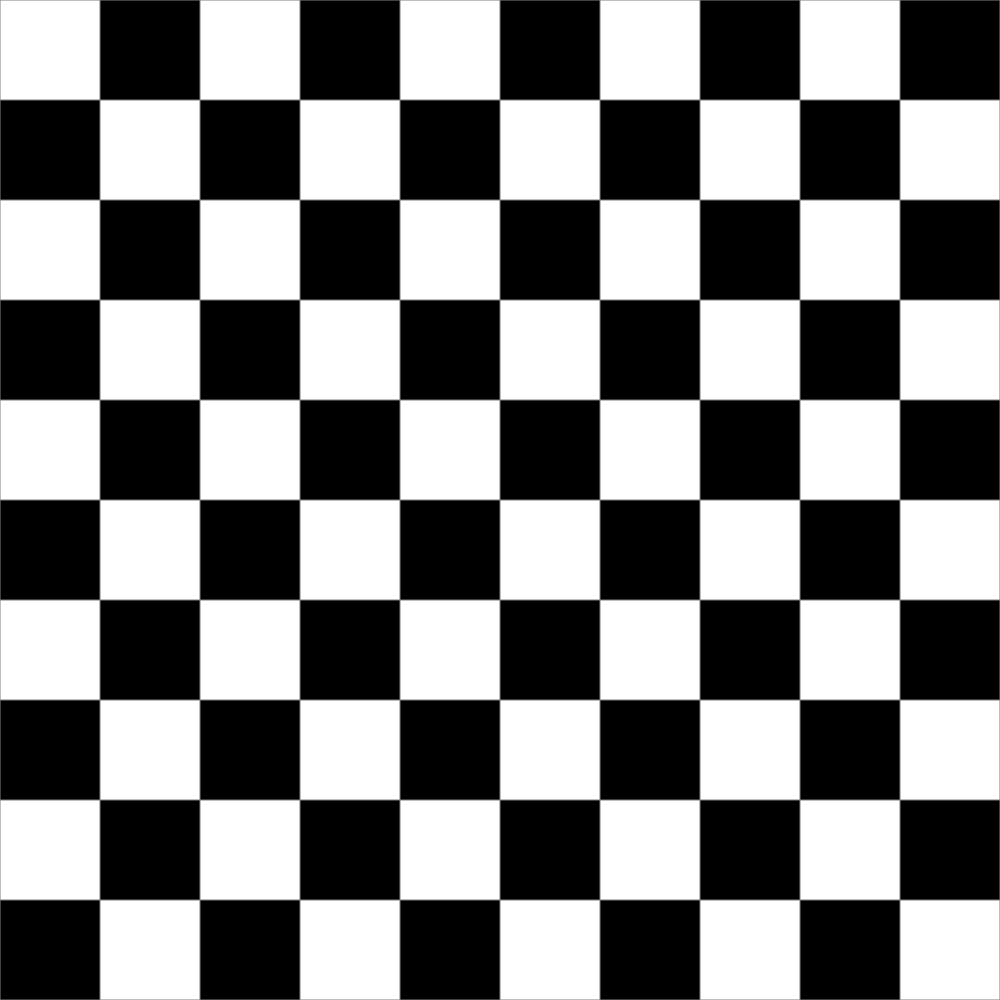
\includegraphics[height = 2in]{../fig/texres.png}
	
	\caption{Each black and white square in this checkerboard represent one texel in the texture applied to the image.  This rendered image demonstrates that the final texture that is rendered contains the full resolution of the desired texture, and that the Blender Internal Renderer is not artificially downsampling the texture.}
	\label{fig:texres}
\end{figure}
